\section{Supervised Learning for Fraud Detection}
    Technique that assumes the availability of historical labelled data. With this technique is possible to identify \textbf{known fraudulent patterns}.\\
    The aim is to build an analytical model predicting a target measure of interest, for example classifying a new instance as fraudulent or not.\\
    The target fraud indicator is usually hard to obtain:
    \begin{itemize}
        \item Typically not provided by the collaborating entity
        \item They are not noise-free, it is crucial to avoid overfitting
    \end{itemize}
    \subsection{Regression vs Classification: Target variables}
    \begin{itemize}
        \item \textbf{Regression}
        \begin{itemize}
            \item Continous target variable
            \item Varies along a predefined limited or unlimited interval 
        \end{itemize}
        \item \textbf{Classification}
        \begin{itemize}
            \item Categorical target variable 
            \item It can only take on a limited set of predefined values
        \end{itemize}
    \end{itemize}
    \subsection{Linear Regression}
        Technique to model a continous target variable.\\
        The goal is to find the \textbf{best fit line} that can accurately predict the output of a continous variable.\\ 
        General formulation:
        $$y(x,w) = w_0 + \sum_{i=1}^{N}w_ix_i$$
        The weights $w_i$ measure the impact on the target variable $y$ of each of the individual explanatory variables.\\
        The weights can be estimated by minimizing a cost function, for example the \textbf{squared error function} (OLS: Ordinary Least Squares).
    \subsection{Logistic Regression (classification)}
        When the target variable is categorical, linear regression gives us no guarantees to have the target in between 0 and 1.\\
        With an S-curved function like the sigmoid, we can bound the values of the target variable.\\
        Logistic regression results can be interpreted as probabilities, the optimization method is Maximum Likelihood Estimation.
    \subsection{Variable Selection}
        Different methods to perform variable selection:
        \begin{itemize}
            \item \textbf{Statistical tests:} to verify if the coefficient of a variable is significantly different from zero, a low p-value represents a significant variable
            \begin{itemize}
                \item Linear Regression: Student's t-distribution 
                \item Logistic Regression: Chi-squared distribution 
            \end{itemize}
            \item \textbf{Forward regression:} start from the empty model and always add variables
            \item \textbf{Backward regression:} start from the full model and always remove variables
            \item \textbf{Stepwise regression:} mix the two
        \end{itemize}
        \subsubsection{Evaluation criteria for variable selection}
            \begin{itemize}
                \item Statistical significance (p-value)
                \item Interpretability
                \item Operational Efficiency 
                \item Legal Issues 
            \end{itemize}
    \subsection{Decision Trees}
        They are recursive-partitioning algorithms, based on a tree-like structure which can represent patterns in an underlying dataset.\\
        Each top node (root node) specifies a testing condition, of which the outcome corresponds to a branch leading up to an internal node. The terminal nodes (leaves) assign fraud labels.\\
        Implement three main functionalities:
        \begin{itemize}
            \item \textbf{Splitting decision}
            \item \textbf{Stopping decision}
            \item \textbf{Assignment decision}
        \end{itemize}
        \subsubsection{Splitting Decision}
            Which variable to split at what value \textit{(e.g. transaction amount is $$>\$100.000$$ or not)}.\\
            To understand the concept, \textbf{impurity or chaos:}
            \begin{itemize}
                \item \textbf{Minimal impurity:} occurs when all customers are either good or bad 
                \item \textbf{Maximal impurity:} occurs when one has the same number of good and bad customers 
            \end{itemize}
            Kinds of impurity measures:
            \begin{itemize}
                \item entropy: bounded in 0 and 1
                \item gini: bounded in 0 and 0.5
            \end{itemize}
            They can be both used with no great differences. The aim of decision tree is to minimize one of these measures (impurity).\\
            By the end of the day the algortim selects a sequence of candidates for a splitting decision and then selects the one that minimizes the impurity.\\
            This approach considers different candidate splits for its root node. It is a greedy and recursive strategy by picking the one with the biggest gain \textit{(gain = decrease in impurity)}.\\
            It can be perfectly parallelized. 
        \subsubsection{Stopping Decision}
            When to stop adding nodes to the tree. If the tree continues to split we'll reach the situation where there is one leaf node per observation (overfitting).\\
            To avoid overfitting train-validation. Stop adding nodes when the validation test curve reaches its minimum.
        \subsubsection{Assignment Decision}
            What class \textit{(fraud/not fraud)} to assign to a leaf node.
    \subsection{Decision Tree Properties}
            \subsubsection{Rule set}
                Decision trees are interpretable models, they can be represented as a rule set: every path from a root node to a leaf makes up a simple if-then rule.\\
                These trees can automatically extract rules, they're a tool which can help experts in build rules: no more manual update.
            \subsubsection{Decision Boundaries}
                Decision tree essentially model decision boundaries orthogonal to the axes
                \begin{figure}[ht!]
                    \centering 
                    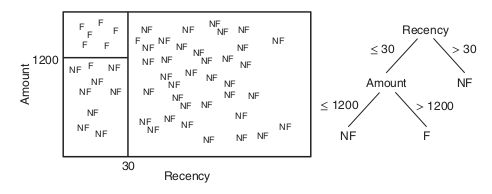
\includegraphics[width=0.6\linewidth]{lecture_15/boundaries.png}
                \end{figure}
    \subsection{Using Decision Trees in Fraud Analytics}
        These mechanisms can be used to interpret the result of other machine learning techniques, for example to interpret clustering solutions:\\
        given the clustering solution, build a decision tree with the cluster output interpreted as label, trying to explain it.\\
        Advantages:
        \begin{itemize}
            \item White-box models with clear explanation: interpretable 
            \item Operationally efficient 
            \item Powerful techniques that allow for more complex decision boundaries than logistic regression 
            \item Non-parametric
        \end{itemize}
        Disadvantage:
        \begin{itemize}
            \item Highly dependent on the sample that was used for tree construction
        \end{itemize}
    \subsection{Neural Networks}
        \textit{Mathematical representations inspired by the functioning of the human brain}.\\
        Can model very complex patterns and decision boundaries in the data. They are a generalization of logistic regression, each neuron uses sigmoid as activation function.
        \subsubsection{MultiLayer Perceptron}
            Sequence of neurons organized in different layers:
            \begin{itemize}
                \item Input layer
                \item Hidden layers 
                \item Output layer 
            \end{itemize}
            Since in fraud analytics there are no complex patterns, neural networks with just one hidden layer are already good.
        \subsubsection{Weights Learning}
            The optimization is more complex: iterative algorithm that optimizes a cost-function
            \begin{itemize}
                \item For regression: MSE 
                \item For classification: Maximum Likelihood 
            \end{itemize}
            Start from a set of random weights, and iteratively adjust them to the patterns in the data using an optimization algorithm (backpropagation).
            The curvature of the objective function is not convex, to avoid local minima start with different randomizations of the weights and select the one with the best performances.\\
            Stop after a certain number of epochs without \textit{progess}.
        \subsubsection{Overfitting}
            Options to mitigate overfitting:
            \begin{itemize}
                \item train test and stop training when you notice an increase of classificaiton error 
                \item weight regularization: put some bound on the value of each weight is going to assume, because neural network work updating weights associated to hidden neurons, bigger weights give importance to something that don't.
            \end{itemize}
        \subsubsection{Variable Selection and Interpretability}
            Neural networks are black box: relate input to output in a mathematically complex, non-transparent and opaque way.\\
            In fraud domain, we need to perform variable selection without removing what can be important to our model: \textbf{Hinton Diagram}.
            The Hinton diagram visualizes the weights between the inputs and the hidden neurons as squares, where the size of the square is proportional to the size of the weight. It is possible to inspect the diagram and remove the variable whose weights are closest to zero.\\
            Another way is to use backward variable selection, by removing features until we start to see a decrease of performance.
        \subsubsection{Rule Extraction Procedure}
            To extract if-then classification rules, mimicking the behavior of the neural network.
            \begin{itemize}
                \item \textbf{Decompositional technique:} decompose the network's internal workings by inspecting weights and/or activation rules.
                \item \textbf{Pedagogical technique:} consider the neural network as a black box and use its predictions as input to a white-box analytical technique such as decision trees.
            \end{itemize}
        \subsubsection{Decompositional Rule Extraction Example}
            \begin{figure}[ht!]
                \centering 
                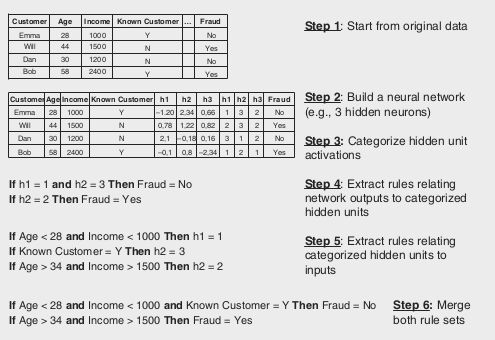
\includegraphics[width=0.6\linewidth]{lecture_15/decompositional.png}
            \end{figure}
        \subsubsection{Pedagogical Rule Extraction Example}
            \begin{figure}[ht!]
                \centering 
                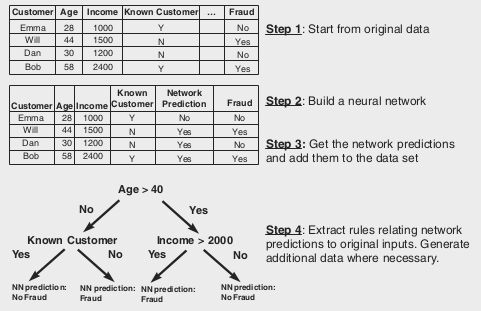
\includegraphics[width=0.6\linewidth]{lecture_15/pedagogical.png}
            \end{figure}
        \subsubsection{Rule Extraction Approaches Evaluation}
            Rule-sets must be evaluated in terms of:
            \begin{itemize}
                \item \textbf{Accuracy}
                \item \textbf{Conciseness}
                \item \textbf{Fidelity:} measures to what extent the extracted rule set succeeds in mimicking the neural network and is calculated as follows.
            \end{itemize}
    \subsection{Two-stage model setup}
        \begin{itemize}
            \item Estimate an easy-to-understand model first \textit{(e.g. linear regression, logistic regression)}, this will give us the interpretability part
            \item Use a neural network to predict the errors made by the simple model using the same set of predictors
            \item Both models are then combined in additive way
        \end{itemize}
        \begin{figure}[ht!]
            \centering 
            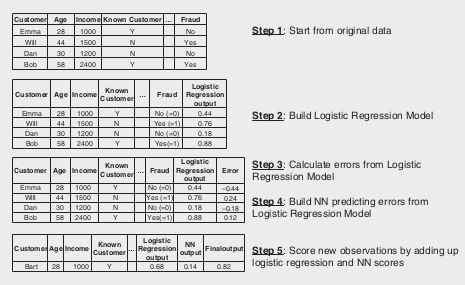
\includegraphics[width=0.6\linewidth]{lecture_15/twostage.png}
        \end{figure}